\begin{sidewaysfigure}[h]
\centering
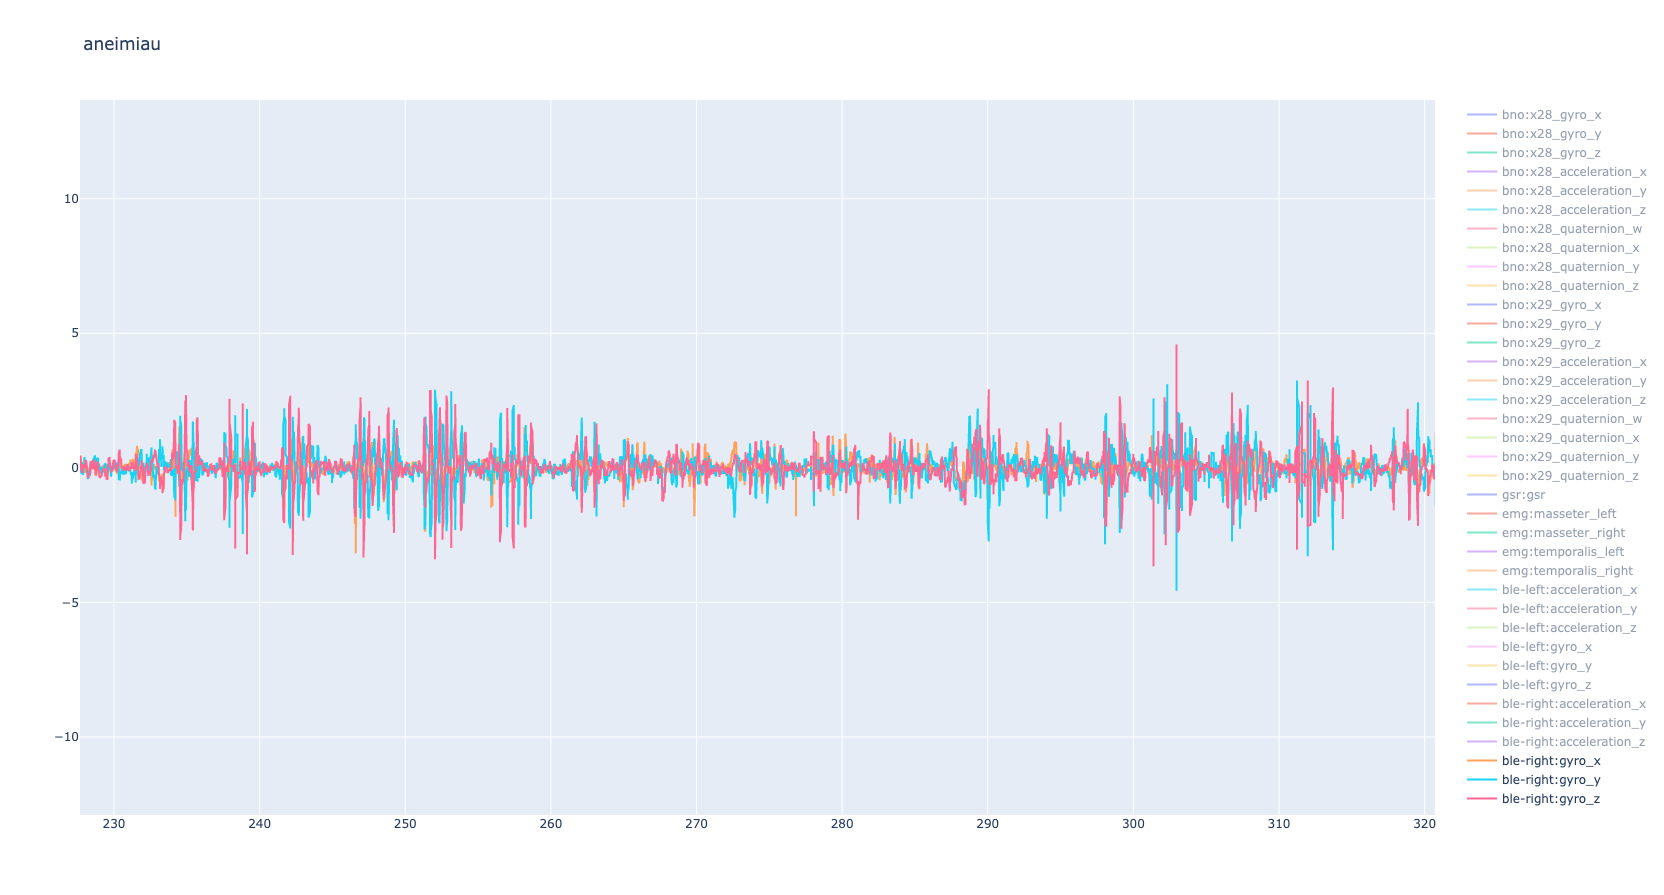
\includegraphics[width=\textwidth]{src/media/study/plots/ble_right_gyro_grind.png}
\caption{Example of a right eSense earable gyroscope x, y, and z time-series slice. The x, y, and z plots are overlapped. From left to right: 3x2s grinding with the right side; 3x4s grinding with the right side; 3x2s grinding with the front side; 3x4s grinding with the front side; 3x2s grinding with all sides; 3x4s grinding with all sides}
\label{plot:ble_right_gyro_grind}
\end{sidewaysfigure}

\begin{sidewaysfigure}[h]
\centering
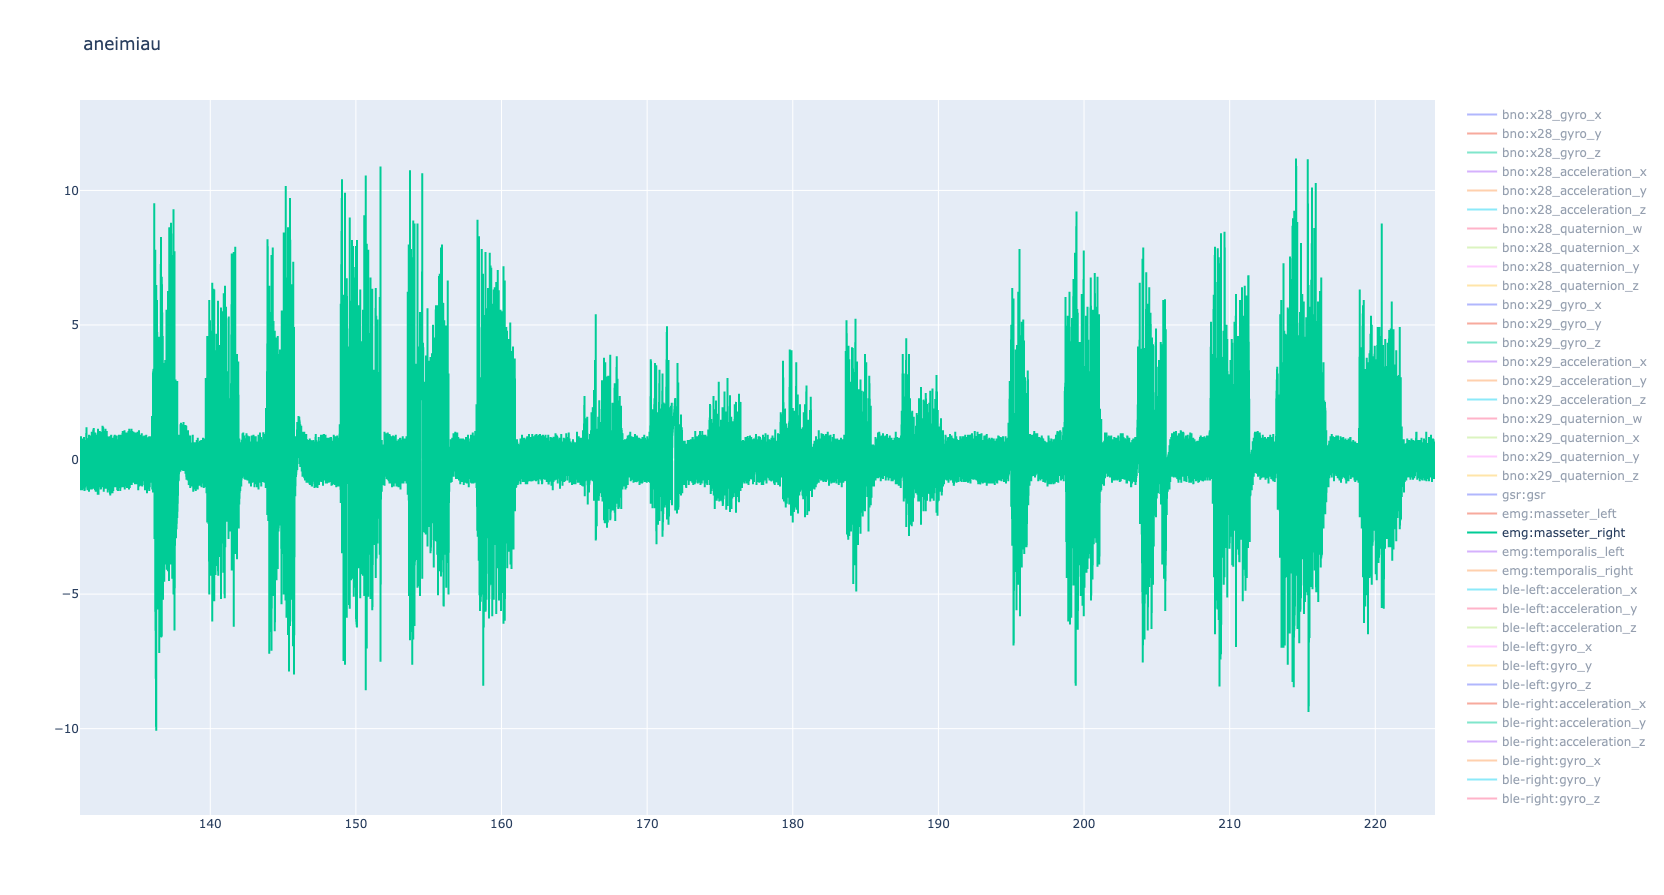
\includegraphics[width=\textwidth]{src/media/study/plots/masseter_right_clenching.png}
\caption{Example of a right masseter time-series slice. From left to right: 3x2s clenching with the right side; 3x4s clenching with the right side; 3x2s clenching with the front side; 3x4s clenching with the front side; 3x2s clenching with all sides; 3x4s clenching with all sides}
\label{plot:masseter_right_clenching}
\end{sidewaysfigure}

\begin{sidewaysfigure}[h]
\centering
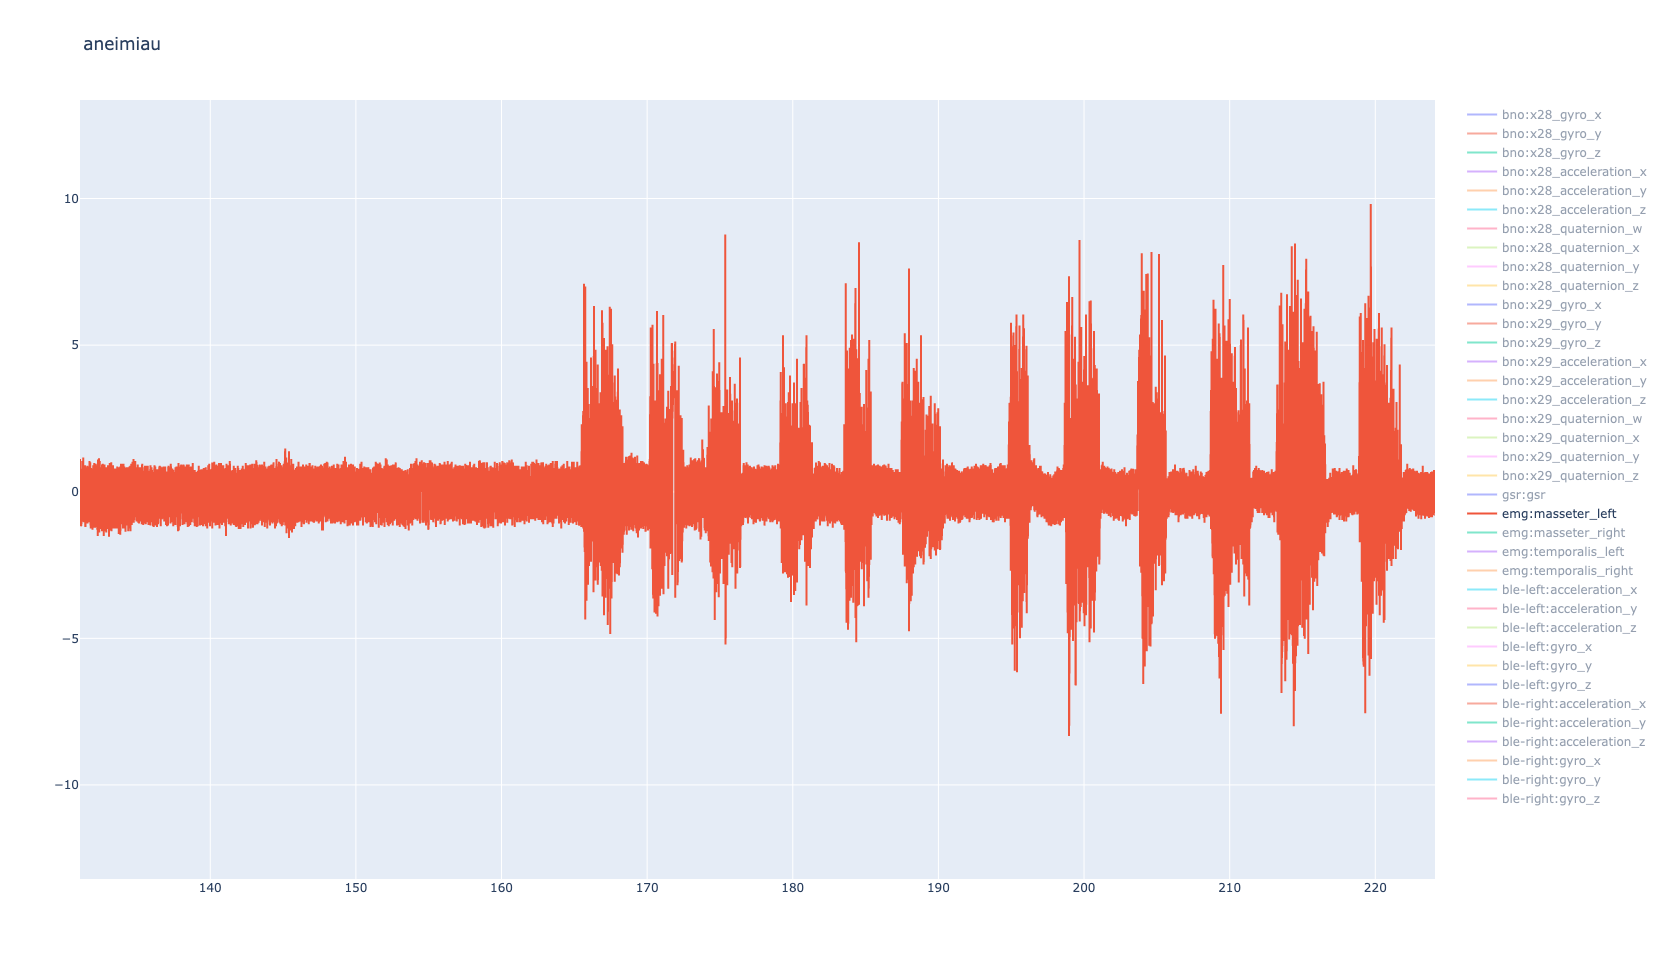
\includegraphics[width=\textwidth]{src/media/study/plots/masseter_left_clenching.png}
\caption{Example of a left masseter time-series slice. From left to right: 3x2s clenching with the right side; 3x4s clenching with the right side; 3x2s clenching with the front side; 3x4s clenching with the front side; 3x2s clenching with all sides; 3x4s clenching with all sides}
\label{plot:masseter_left_clenching}
\end{sidewaysfigure}

\begin{sidewaysfigure}[h]
\centering
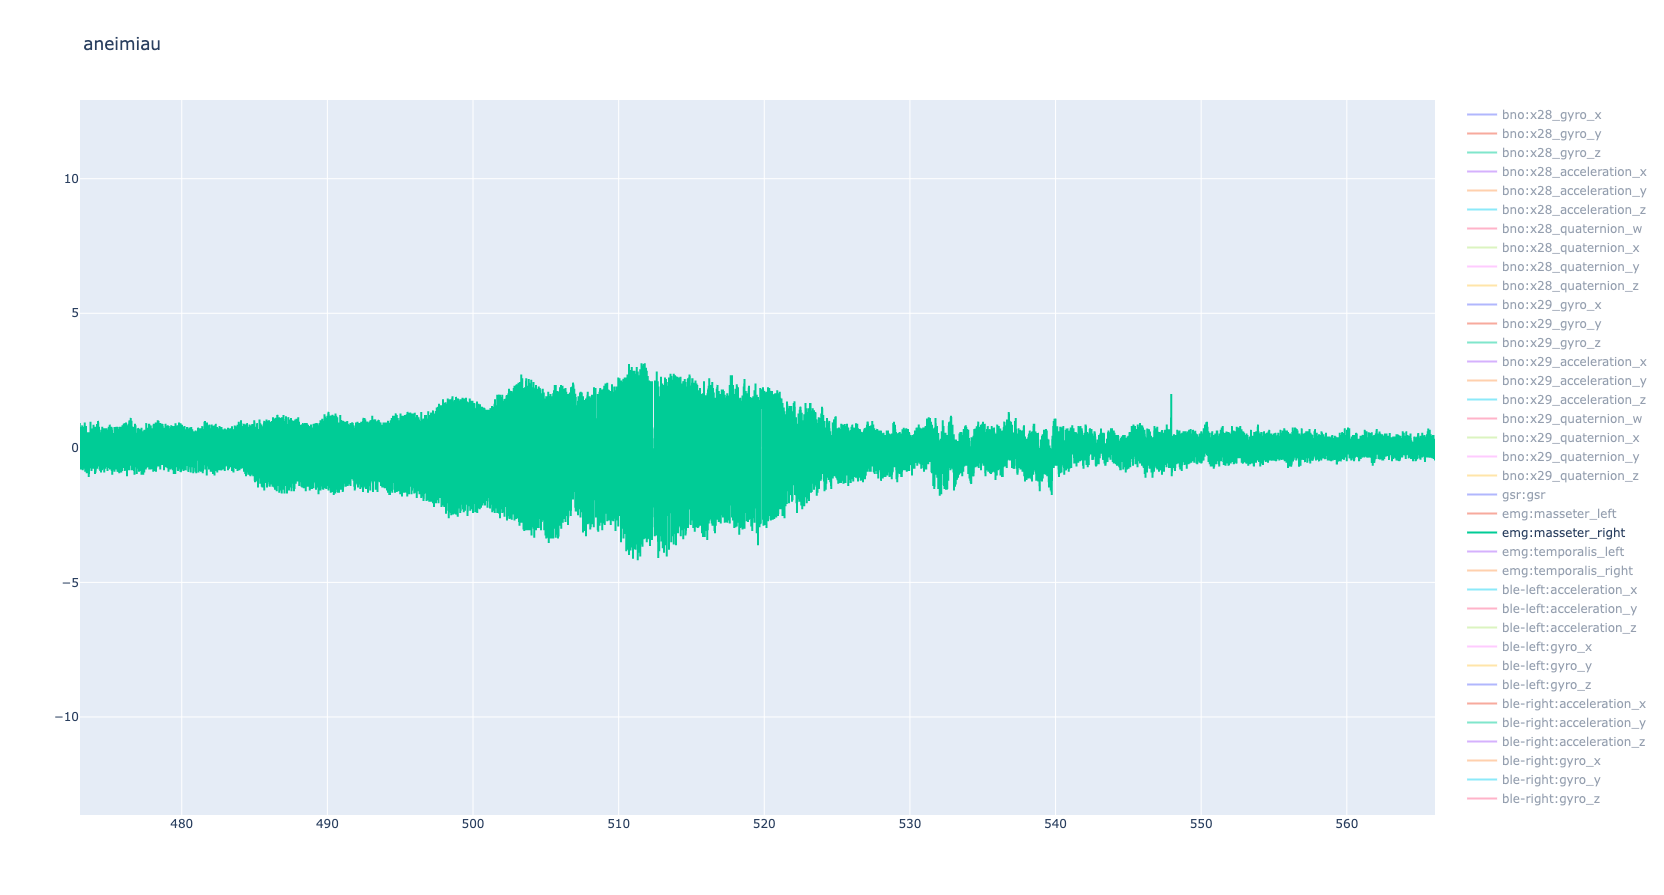
\includegraphics[width=\textwidth]{src/media/study/plots/masseter_right_talking.png}
\caption{Example of a right masseter time-series slice. Reading}
\label{plot:masseter_reading}
\end{sidewaysfigure}

\begin{sidewaysfigure}[h]
\centering
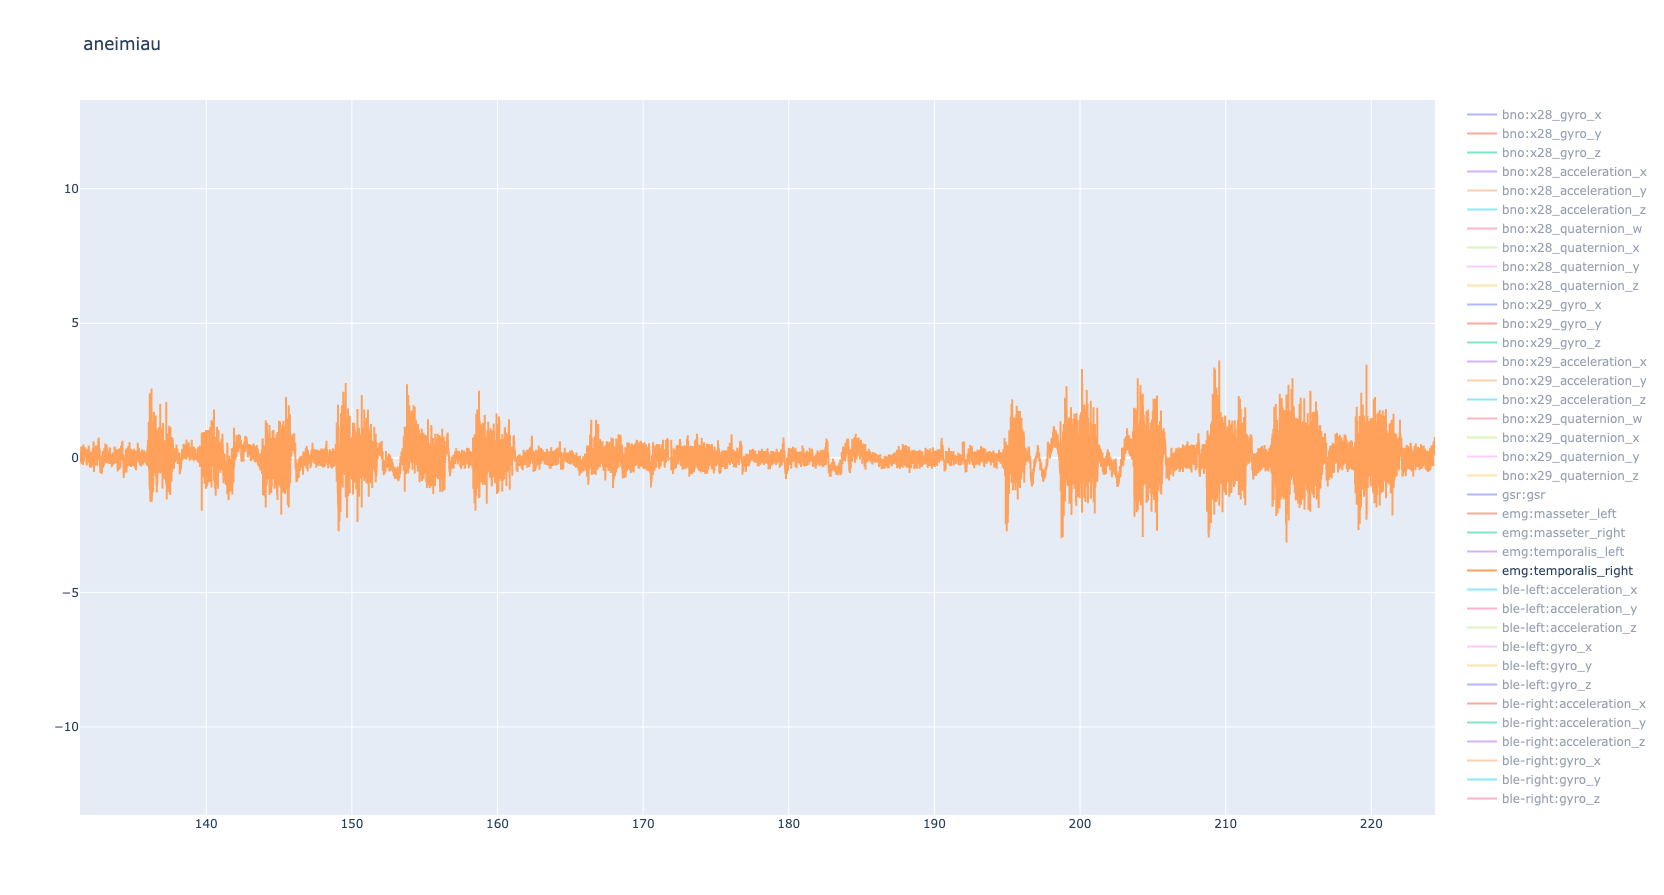
\includegraphics[width=\textwidth]{src/media/study/plots/temporalis_right.png}
\caption{Example of a right temporalis time-series slice. From left to right: 3x2s clenching with the right side; 3x4s clenching with the right side; 3x2s clenching with the front side; 3x4s clenching with the front side; 3x2s clenching with all sides; 3x4s clenching with all sides}
\label{plot:temporalis_right}
\end{sidewaysfigure}

\begin{sidewaysfigure}[h]
\centering
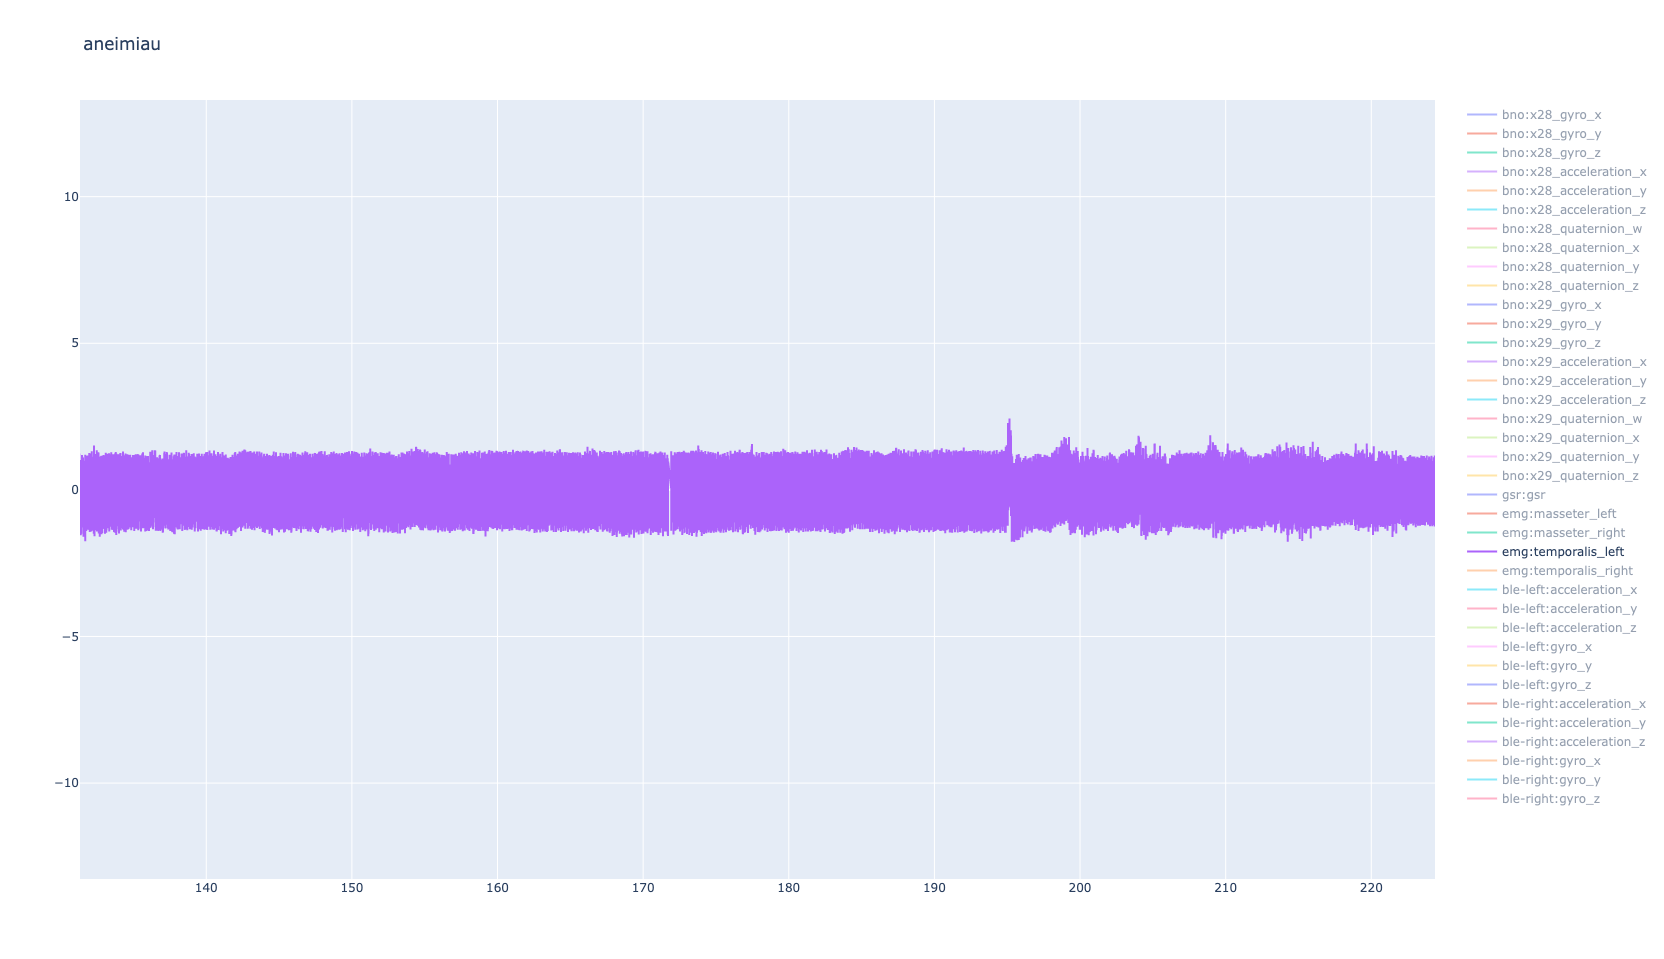
\includegraphics[width=\textwidth]{src/media/study/plots/temporalis_left.png}
\caption{Example of a left temporalis time-series slice. From left to right: 3x2s clenching with the right side; 3x4s clenching with the right side; 3x2s clenching with the front side; 3x4s clenching with the front side; 3x2s clenching with all sides; 3x4s clenching with all sides. Note that it's not possible to differentiate between the performed exercises here.}
\label{plot:temporalis_left}
\end{sidewaysfigure}

\begin{sidewaysfigure}[h]
\centering
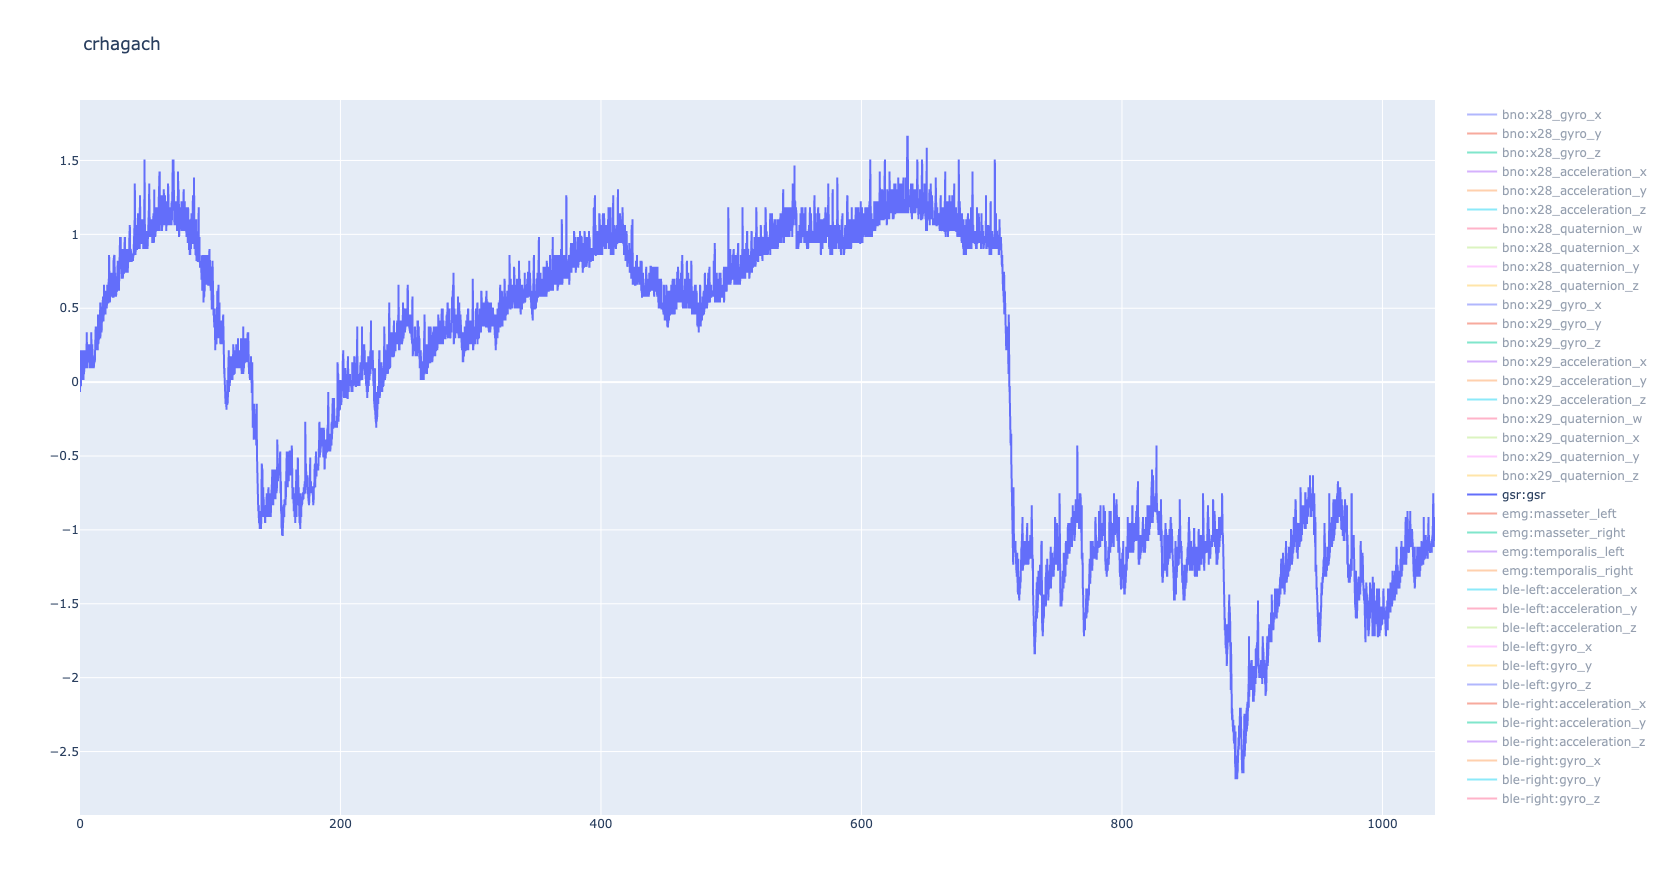
\includegraphics[width=\textwidth]{src/media/study/plots/gsr.png}
\caption{Example of a GSR time-series}
\label{plot:gsr}
\end{sidewaysfigure}

\begin{sidewaysfigure}[h]
\centering
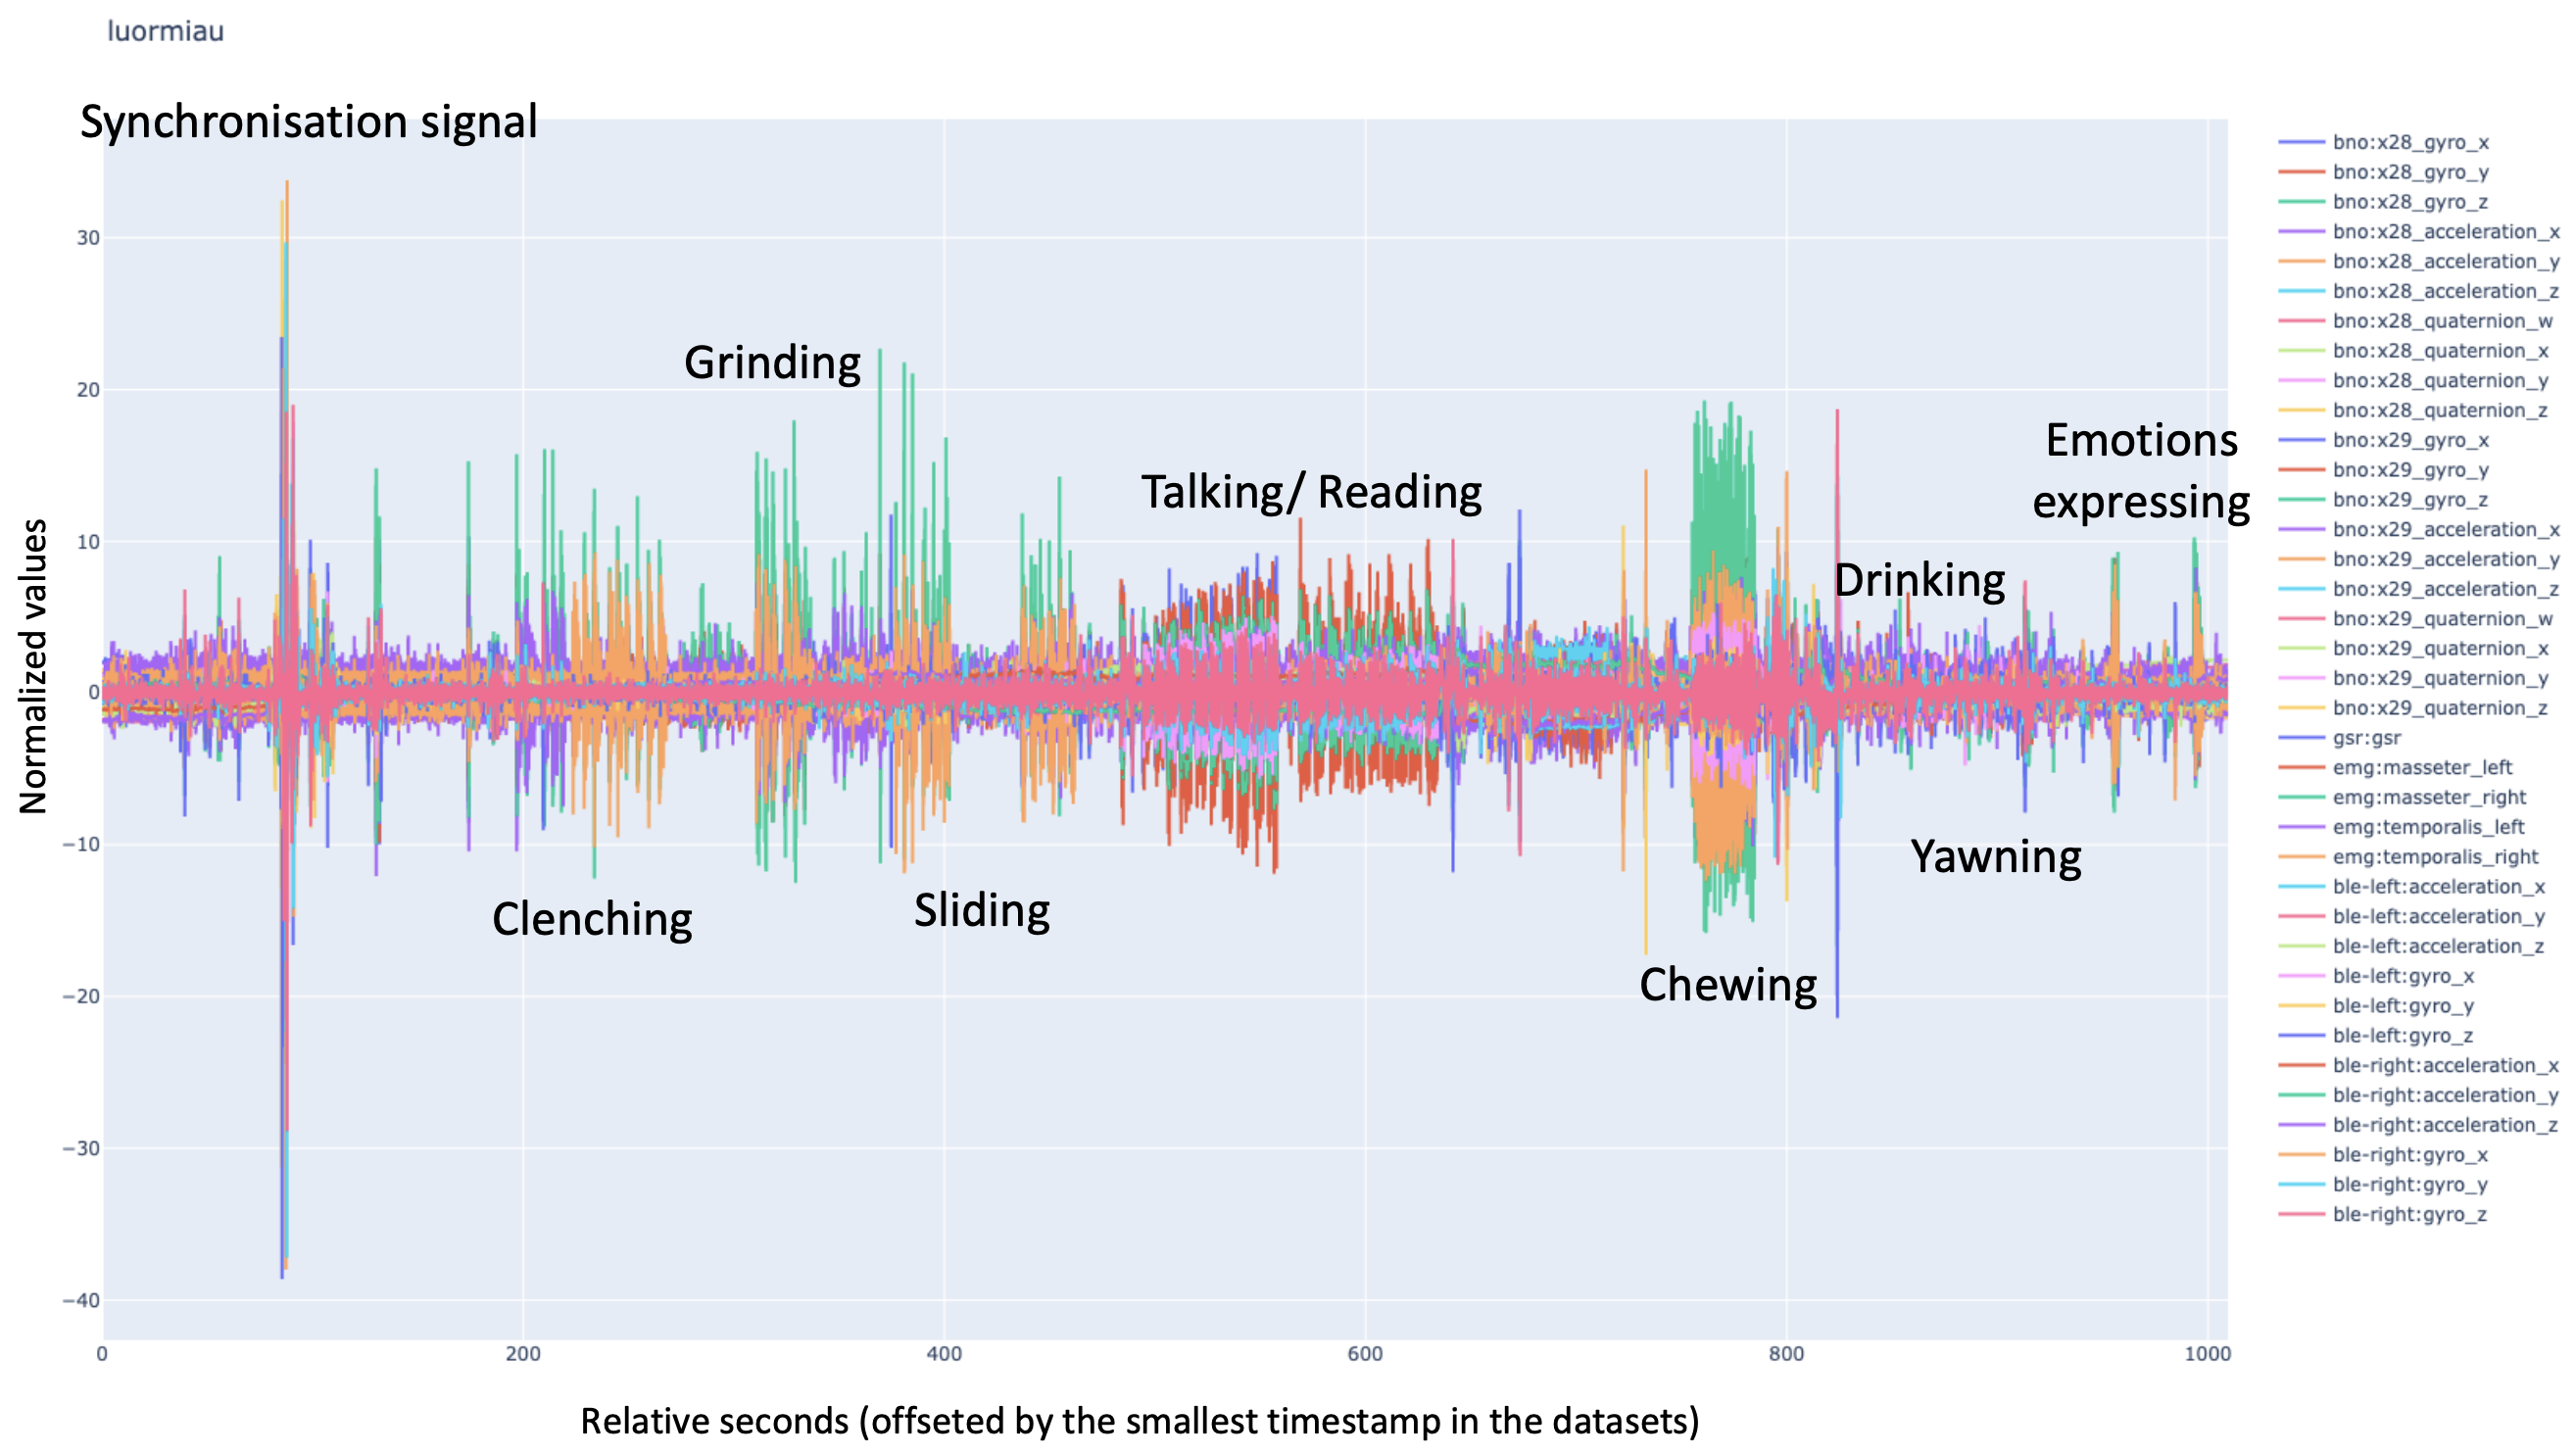
\includegraphics[width=\textwidth]{src/media/methodology/overview.png}
\caption{Overview of a normalized dataset}
\label{image:dataset_overview}
\end{sidewaysfigure}